%!TEX encoding = UTF-8 Unicode
% -*- coding: UTF-8; -*-
% vim: set fenc-utf-8

\chapter{Diagrammes de séquence de conception}
\label{s:sequence_conception}

Ce chapitre présente les diagrammes de séquence de conception associée aux fonctionnalitées de l'application.

\section{Convertir les coordonnées de la souris en coordonnées réelles}
\label{sec:convertir_coordonnees_souris}

%\begin{figure}[htpb]
%    \centering
%    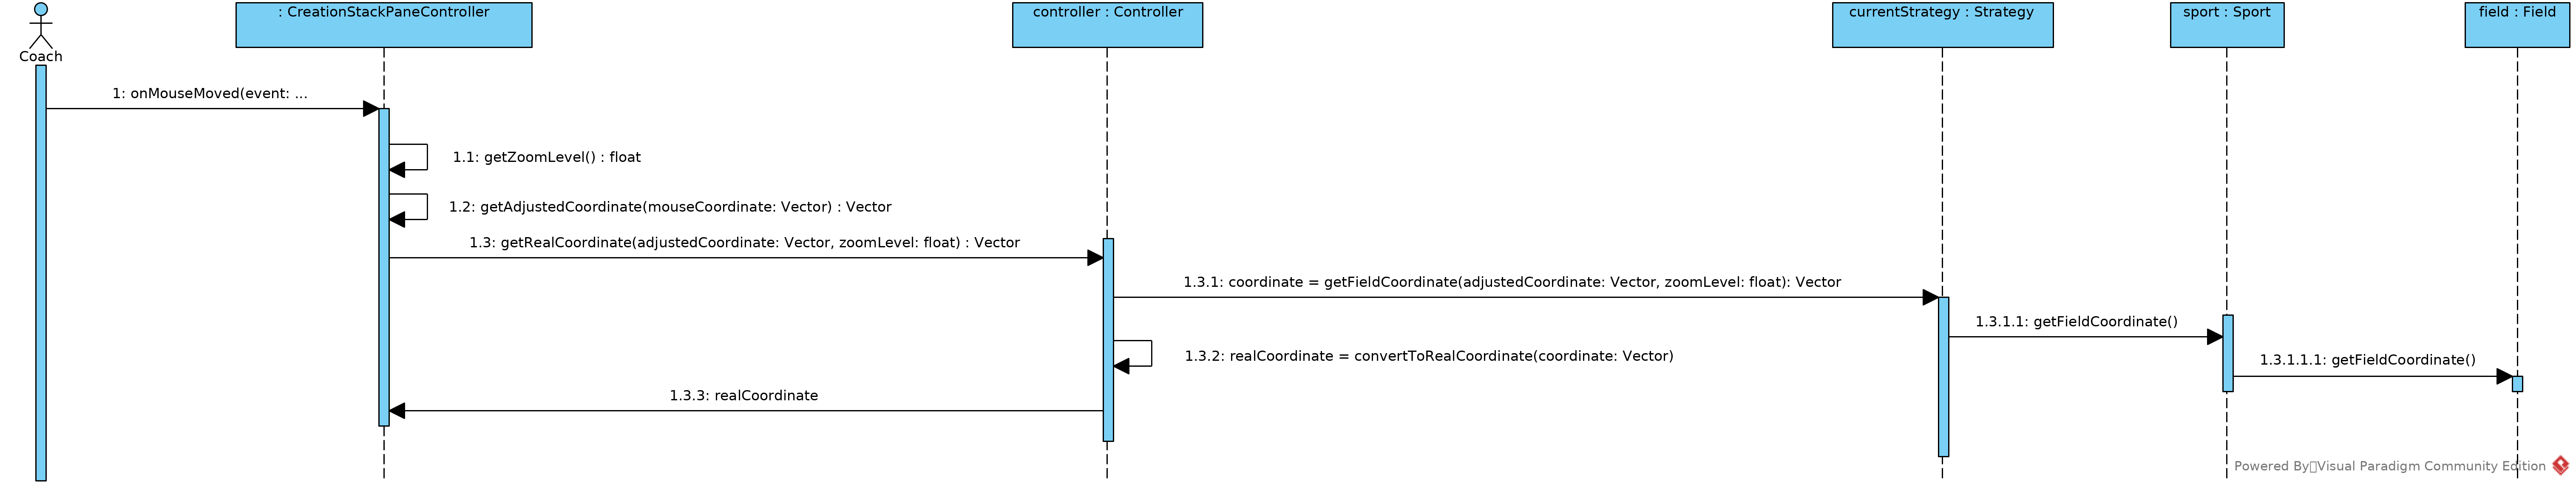
\includegraphics[scale=0.7]{fig/dsc_getRealCoordinate.png}
%    \caption{Diagramme de séquence de conception pour Convertir les coordonnées de la souris en coordonnées réelles}
%    \label{fig:dsc_pixel_reel}
%\end{figure}

La figure \ref{fig:dsc_pixel_reel} est le diagramme de séquence pour obtenir les coordonées réelles à partir des coordonnées de la souris.
La fenêtre reçoit un événement lors du déplacement de la souris.
Elle récupère le niveau de zoom actuel et ajuste les coordonnées de la souris selon le déplacement horizontal et vertical du terrain.
Le contrôleur est appelé, qui délègue l'appel pour obtenir les coordonées du terrain à la stratégie courante.
Une fois les coordonnées du terrain obtenues, elles sont converties en coordonnées réelles (e.g: en mètre) et retournées.


\section{Ajouter un joueur}
\label{sec:ajouter_joueur}

%\begin{figure}[htpb]
%    \centering
%    \includegraphics[scale=0.7]{fig/dsc_createPlayer.png}
%    \caption{Diagramme de séquence de conception pour ajouter un joueur sur le terrain}
%    \label{fig:dsc_create_player}
%\end{figure}

La figure \ref{fig:dsc_create_player} est le diagramme séquence lorsqu'un nouveau joueur est ajouté sur le terrain.
La fenêtre reçoit un événement lorsque que la souris est en mode \textit{Glisser}.
L'ajout d'un joueur se fait lorsque l'utilisateur dépose celui-ci sur le terrain.
Le contrôleur est alors appelé et il crée un identifiant pour le nouveau joueur,
Puis, ce joueur est ajouté dans le domaine, ainsi que dans l'image courante.


%\begin{figure}[htpb]
%    \centering
%    \includegraphics[scale=0.7]{fig/dsc_dragPlayer.png}
%    \caption{Diagramme de séquence de conception pour déplacer un joueur sur le terrain}
%    \label{fig:dsc_drag_player}
%\end{figure}

La figure \ref{fig:dsc_drag_player} est le diagramme de séquence lorqu'un joueur est déplacé à un nouvel endroit sur le terrain.
La sélection du joueur sur le terrain est expliqué en détail à la section \ref{sec:convertir_clic_en_objet}.

\section{Sélectionner l'objet de jeu sous la souris après un clic}
\label{sec:convertir_clic_en_objet}

%\begin{figure}[htpb]
%    \centering
%    \includegraphics[scale=0.7]{fig/dsc_getGameObject.png}
%    \caption{Diagramme de séquence de conception pour obtenir l'objet de jeu sous la souris après un clic}
%    \label{fig:dsc_get_game_object}
%\end{figure}

La figure \ref{fig:dsc_get_game_object} est le diagramme de séquence pour sélectionner l'objet de jeu sous la souris.
Les coordonnées du terrain sont obtenus en délégant l'appel à la stratégie courante.
L'image actuelle de la stratégie est récupérée et l'objet \textit{Frame} est appelée.
Celui-ci parcours tous les objets de jeu qu'il contient, puis calcul la distance entre les coordonnées et l'objet de jeu.
Si la distance est inférieur aux valeurs de dimensions en x ou en y, l'identifiant de cet objet de jeu est retourné.
Autrement, un identifiant \textit{null} est retourné.

\section{Édition en mode image par image}
\label{sec:edition_image_par_image}

%\begin{figure}[htpb]
%    \centering
%    \includegraphics[scale=0.7]{fig/dsc_editImageByImage.png}
%    \caption{Diagramme de séquence de conception pour le mode d'édition image par image}
%    \label{fig:dsc_edit_image}
%\end{figure}

La figure \ref{fig:dsc_edit_image} est le diagramme de séquence des différentes intéractions entre le système et l'utilisateur lors de l'édition d'une stratégie en mode \textbf{image par image}.
Lorsque l'utilisateur change pour ce mode d'édition, la fenête principale s'occupe d'initialiser les éléments de la vue.
Si l'utilisateur clique sur un joueur et le déplace, les scénarios pour obtenir la sélection sous la souris \ref{sec:convertir_clic_en_objet} et déplacer un joueur \ref{sec:ajout_joueur} sont exécutés.
Par soucis de lisibilité, tous les appels ne sont pas reproduits.

Lorsque l'utilisateur clique sur «prochaine image», la fenêtre sauvegarde les informations actuelles, puis appelle le contrôleur pour obtenir la prochaine image.
S'il n'y a pas de prochaine image, une nouvelle est créée en copiant les informations de l'image actuelle.
La vue rend transparentes les informations de l'ancienne image et affiche la nouvelle image.

Lorsque l'utilisateur clique sur «image précédente», la fenêtre récupère à l'aide du contrôleur les deux dernières images.
Si l'une des deux images n'existe pas, null est retourné.
La plus ancienne des deux images est affichée avec un niveau de transparence et l'image immédiatement précédente à celle en cours est affichée.

En mode << suppression >>, lorsque l'utilisateur clique sur un objet de jeu, le scénario pour obtenir la sélection, \ref{sec:convertir_clic_en_objet}, est exécuté.
Ensuit, un appel au contrôleur est fait pour supprimer l'objet avec l'identifiant acquis.
Cet appel est uniquement exécuté si l'identifiant n'est pas null.

\section{Édition en mode temps réel}
\label{sec:edition_temps_reel}

%\begin{figure}[htpb]
%    \centering
%    \includegraphics[scale=0.7]{fig/dsc_editRealTime.png}
%    \caption{Diagramme de séquence de conception pour le mode d'édition en temps réel}
%    \label{fig:dsc_edit_real_time}
%\end{figure}

La figure \ref{fig:dsc_edit_real_time} est le diagramme de séquence des différentes intéractions entre le système et l'utilisateur lors de l'édition d'une stratégie en mode \textbf{temps réel}.
Ce mode est très similaire avec celui image par image (\ref{sec:edition_impage_par_image}).
La différence principale est que lorsque l'utilisateur exécute le scénario pour déplacer un joueur (\ref{sec:ajout_joueur}), plusieurs appels supplémentaires doivent être faits.
Lorsqu'un déplacement est débuté, un booléen est modifié à Vrai (\textit{setRealTimeDrag()}).

À chaque événement de déplacement de la souris, les appels nécessaires pour positionner le joueur sont faits.
Plutôt que de positionner dans une image, la position est mise dans une \textbf{sous-image}.
Cette sous-image est retournée et affichée.
Ceci permet de rejouer les mouvements depuis la dernière image des joueurs.

Lorsque le déplacement est terminé, le booléen est modifié à Faux (\textit{unsetRealTimeDrag()}) et la fenêtre met fin au mode de déplacement en temps réel.
L'édition en temps réel peut se poursuivre.

\section{Visionner le jeu}
\label{sec:visionner_jeu}

%\begin{figure}[htpb]
%    \centering
%    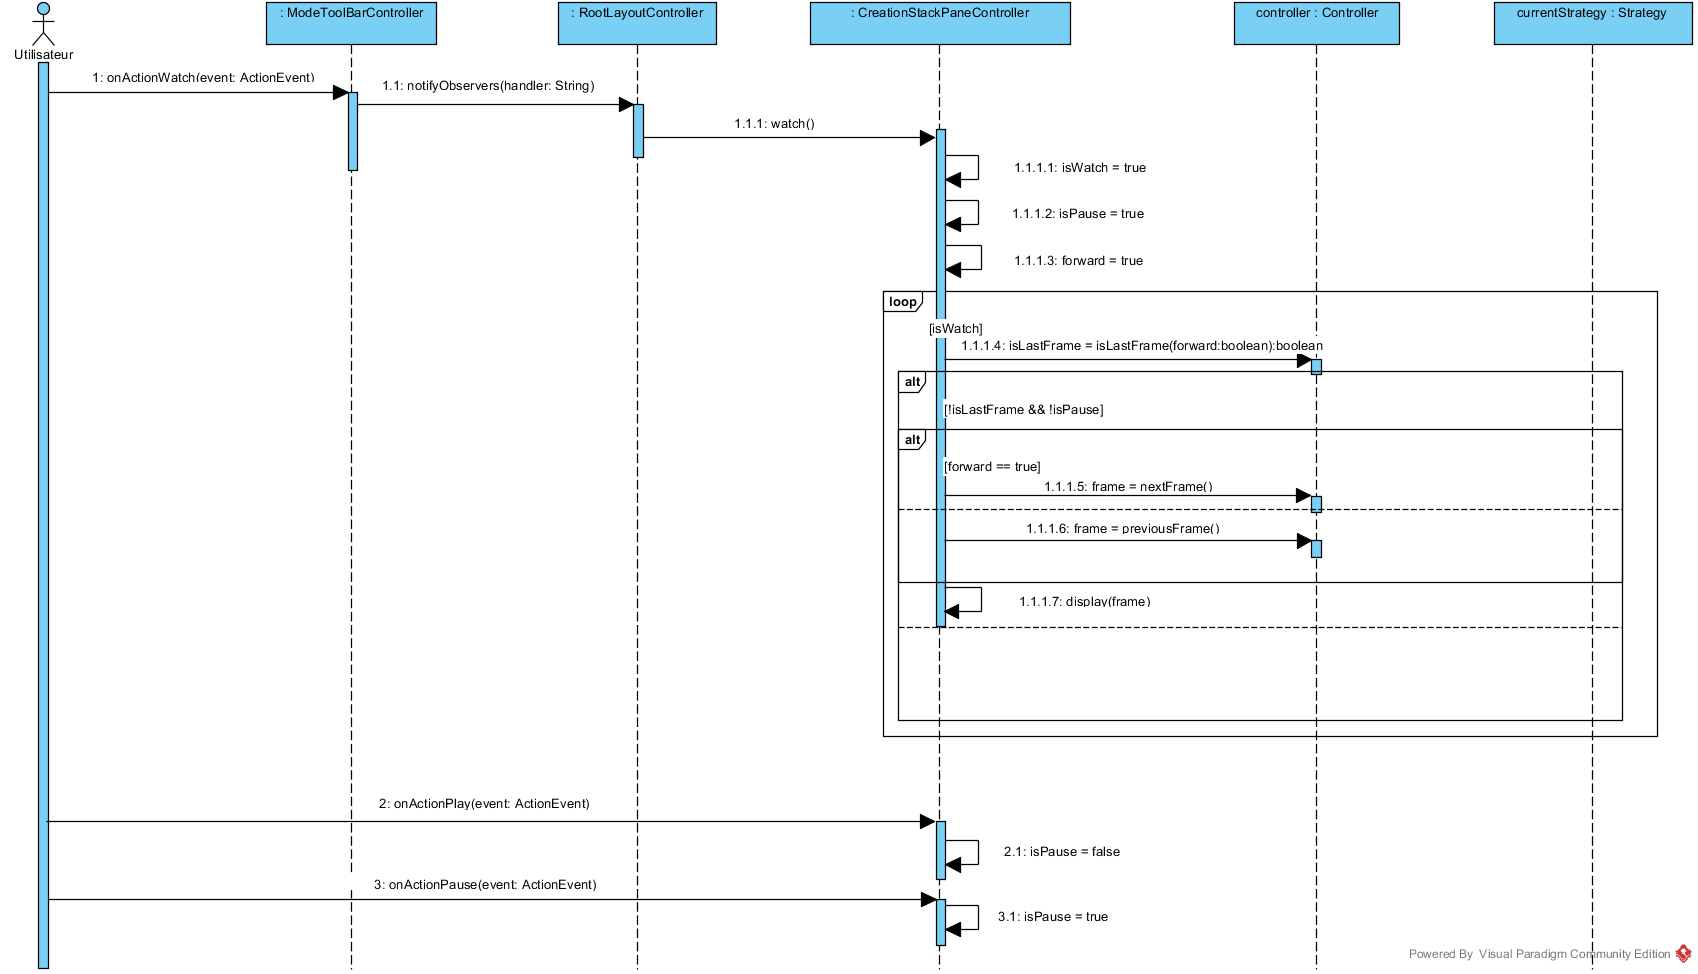
\includegraphics[scale=0.7]{fig/dsc_visionnement_watch.png}
%    \caption{Diagramme de séquence de conception pour le mode de visionnement (partie principale)}
%    \label{fig:dsc_view_main}
%\end{figure}

La figure \ref{fig:dsc_view_main} est le diagramme de séquence pour les principales intéractions lors du visionnement.

Lorsque l'utilisateur passe en mode visionnement, le système entre dans une boucle gouvernée par un booléen: \textbf{isWatch}.
Par défaut, le visionnement est sur pause.
Si l'utilisateur active le visionnement, le booléen: \textbf{isPause} est mis à Faux.
Si l'utilisateur met sur pause, ce même booléen est mis à Vrai.
À chaque itération de la boucle, le système récupère une image.
Si le visionnement n'est pas sur pause ou si la dernière image affichée n'était pas la dernière image disponible, le système affiche l'image.

%\begin{figure}[htpb]
%    \centering
%    \includegraphics[scale=0.7]{fig/dsc_visionnement_edit_index.png}
%    \caption{Diagramme de séquence de conception pour le mode de visionnement (modification du temps)}
%    \label{fig:dsc_view_edit_idx}
%\end{figure}

La figure \ref{fig:dsc_view_edit_idx} est le diagramme de séquence lorsque l'utilisateur souhaite avancer ou reculer d'un temps ajustable.
Lorsque le temps est saisi, le système appel le contrôleur pour ajuster le temps actuel.
Le contrôleur est responsable de traduire le différentiel de temps en un différentiel d'images et il tente de modifier autant que possible l'image en cours.
La nouvelle image actuelle est retournée et affichée.

%\begin{figure}[htpb]
%    \centering
%    \includegraphics[scale=0.7]{fig/dsc_visionnement_forward.png}
%    \caption{Diagramme de séquence de conception pour le mode de visionnement (avancement rapide)}
%    \label{fig:dsc_view_forward}
%\end{figure}

La figure \ref{fig:dsc_view_forward} est le diagramme de séquence lorsque l'utilisateur souhaite avancer en accélérer la stratégie.
Le sens est vérifié et si le visionnement se faisait en reculant, la vitesse de visionnement est remise à sa valeur par défaut.
La vitesse est accélérée en appelant le contrôleur.

%\begin{figure}[htpb]
%    \centering
%    \includegraphics[scale=0.7]{fig/dsc_visionnement_rewind.png}
%    \caption{Diagramme de séquence de conception pour le mode de visionnement (reculuement rapide)}
%    \label{fig:dsc_view_rewind}
%\end{figure}

La figure \ref{fig:dsc_view_rewind} est le diagramme de séquence lorsque l'utilisateur souhaite reculer en accélérer la stratégie.
C'est la même logique que dans le cas de l'avancement rapide, mais modifié pour tenir compte du sens de visionnement renversé.
